\documentclass[main.tex]{subfiles}

\begin{document}

\chapter{Post Assembly} \label{chapter:postassembly}


\subsection{Trouble with heuristic algorithm}

Due to memory constraint and cpu usage you can't build and store all overlap.
Due to theoretical limit, how many of base need to be share between to read to create an overlap how many error we can accept in this overlap.

Assembly tools need use heuristic algorithm, solve assembly trouble in this constraint, in majority of case this heuristic perform a very good work, but in some case we need perform a more complex analysis.

\citeauthor{long_read_assembler_comparison} in \cite{long_read_assembler_comparison} perform a comparison of five assembly tools on real data and simulated data bacterial data set. Some trouble in long-reads was simulated to stress assembly tools:
\begin{itemize}
    \item adaptator length, sequencing require add short sequence before reads, remove this adaptator in long-read sequencing technology aren't trivial
    \item chimeric read, during DNA extraction and fragmentation two fragment come from different region an can lead to assembly fragmentation
    \item glitch level, long-read error aren't uniformly distributed along the reads and sometimes sequencer create a region with only random sequence. A more important the glitch level indicate the bigger the glitch will be and the more frequently it will happen
    \item random junk read, some read are just a string of random character
    \item read depth, correspond to genome coverage
    \item read identity, percent of error insertion, deletion, substitution 
    \item read length, length of read 
\end{itemize}

\begin{figure}
    \centering
    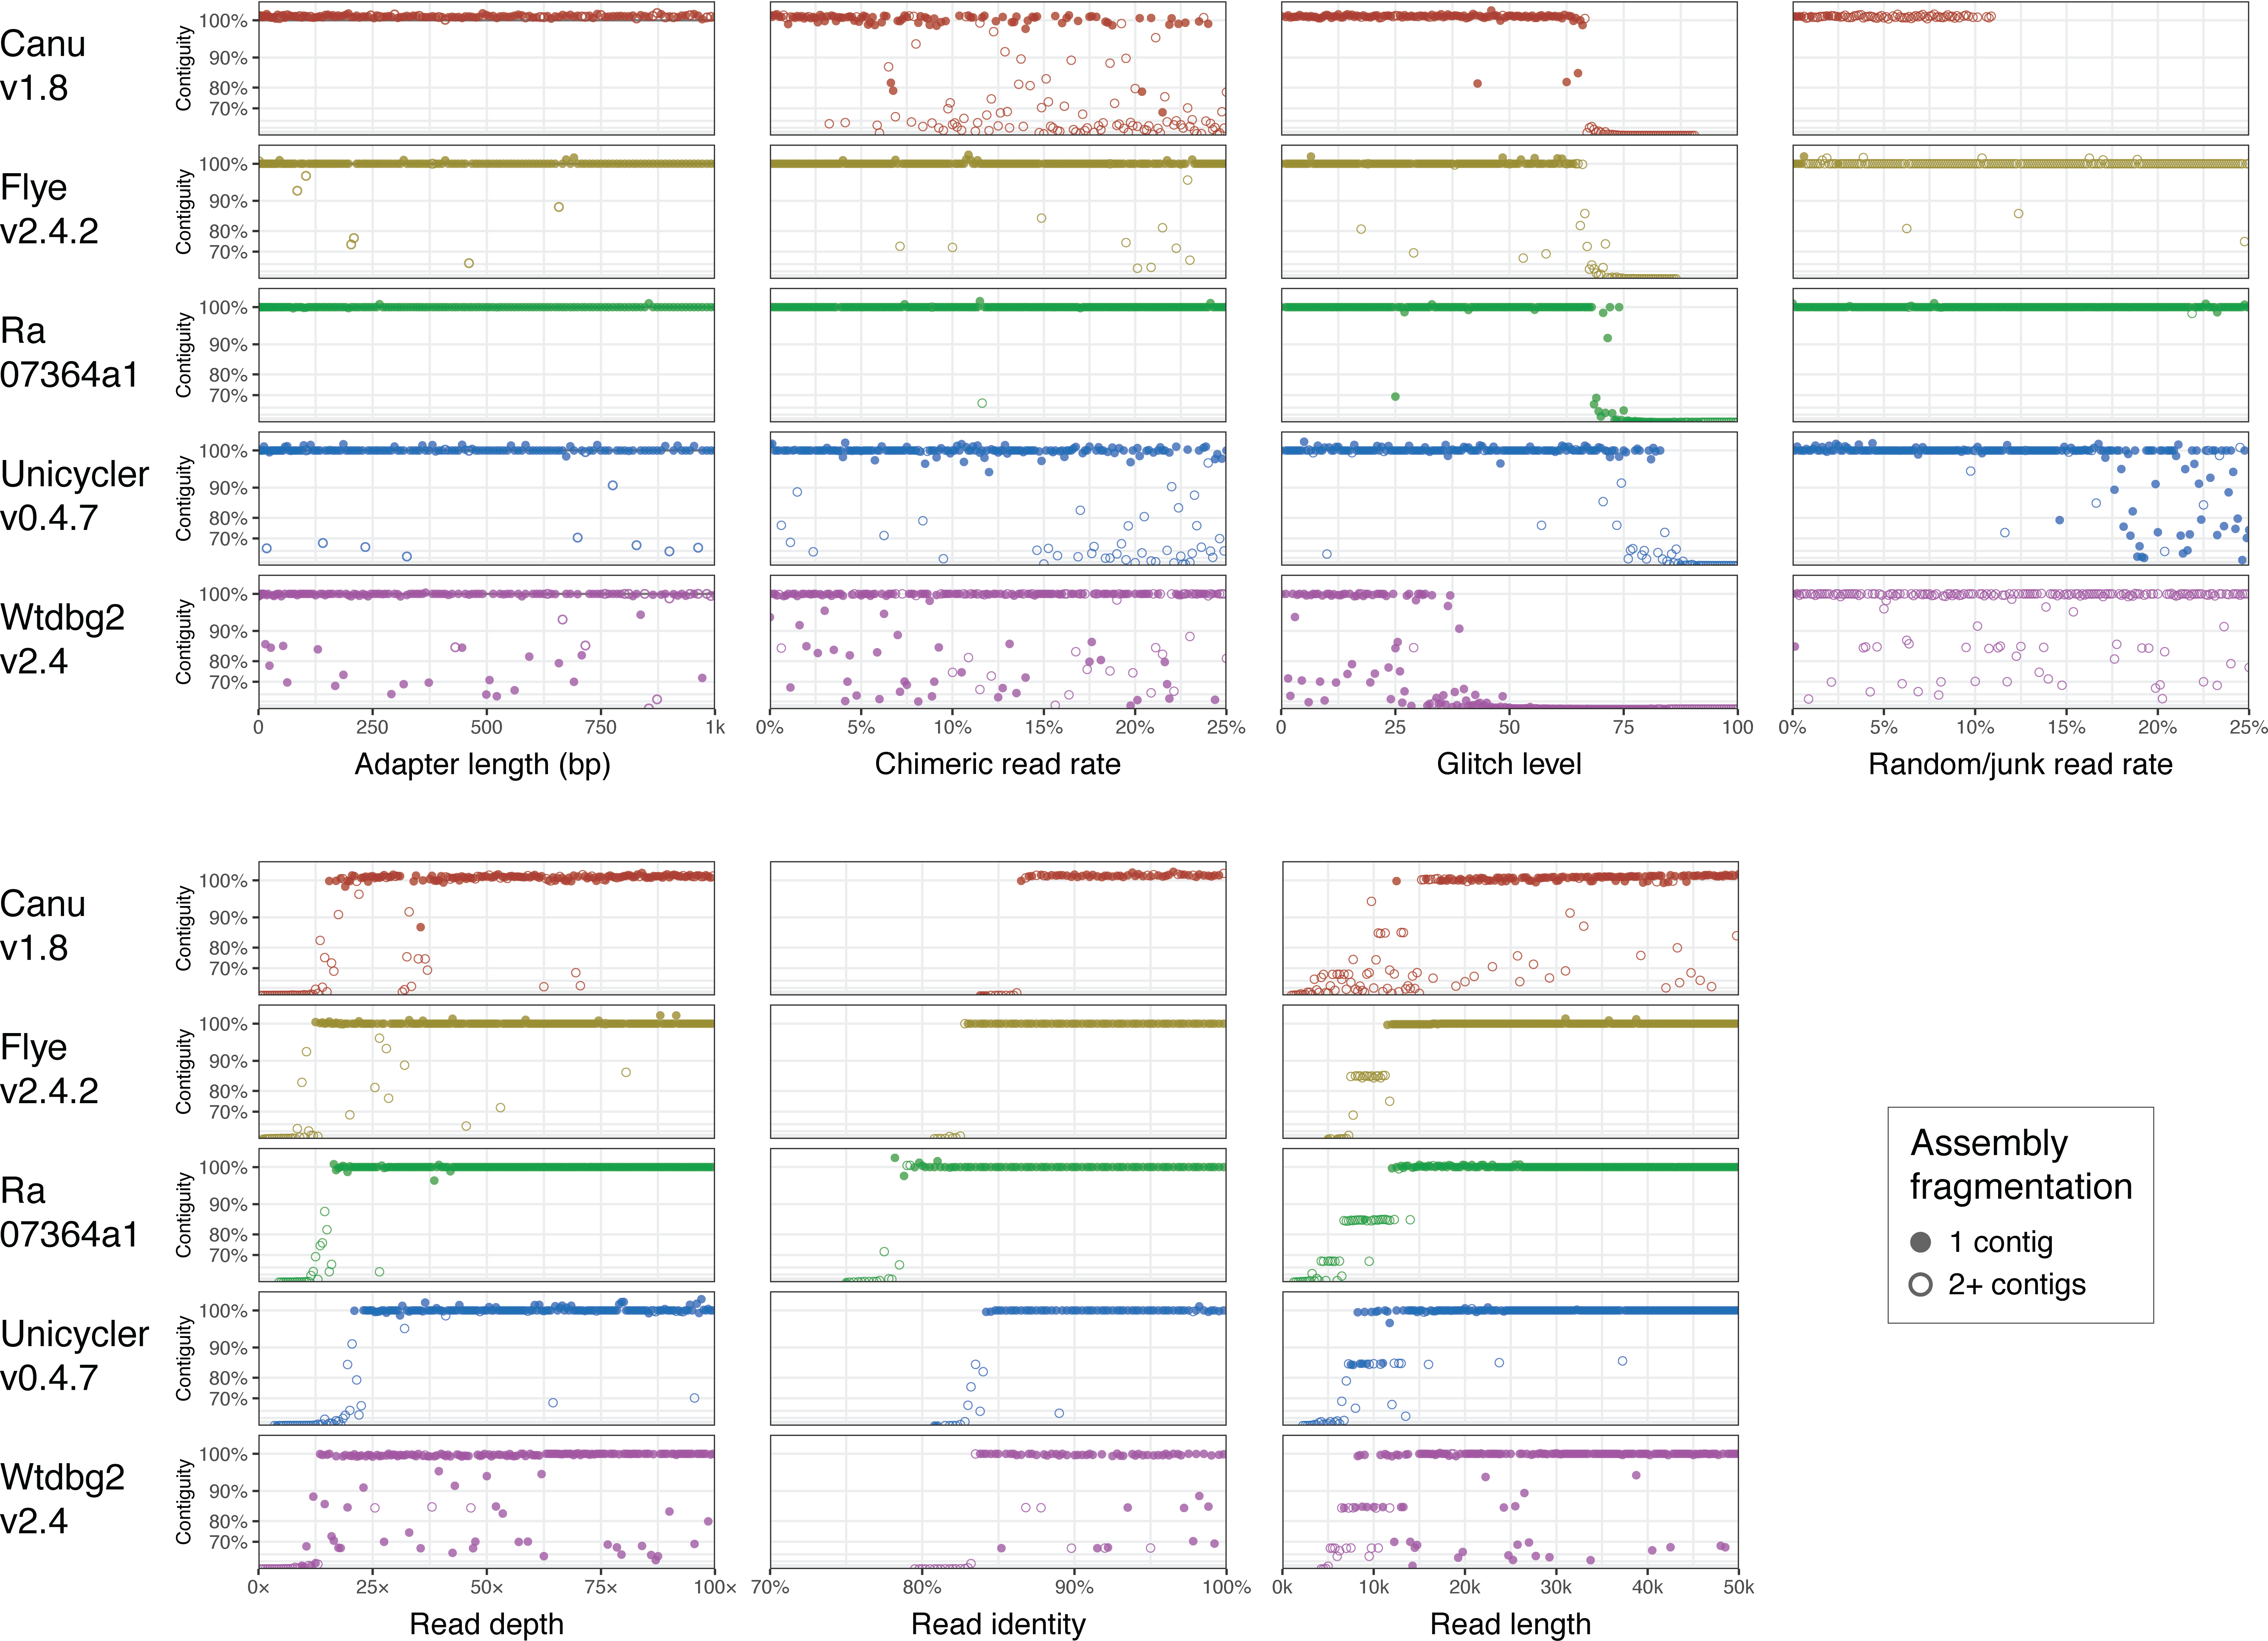
\includegraphics[width=\textwidth]{introduction/images/rrwick_bench.png}
    \caption{Effect of different reads property on assembly contiguity (number of contigs expect and map correctly on reference genome), of five assembly tools, \toolsname{Unicycler} was an hybrid assembler (use second and thrid generation read), \canu was a long-read assembly pipeline they perform a self correction before construct assembly with a special \OLC graph (more detail in Section \ref{section:sota:canu}), \toolsname{Ra} perform a basic string graph assembly on raw reads with a correction of contigs after assembly (more detail in Section \ref{section:sota:miniasm}), \wtdbg and \toolsname{Flye} use a \DBG like approach to perform assembly on raw reads (more detail in Section \ref{section:sota:wtdbg}). This figure was a reproduction of figure from \cite{long_read_assembler_comparison}.}
    \label{intro:fig:rrwick_bench}
\end{figure}

This study focus on contiguity of assembly, if the number of contig match with the expected number of contig and if this contigs map against the reference. All assembly perform a good assembly when:
\begin{itemize}
    \item reads length are upper than 10k and lower than 20k, this length was reach by long-read sequencing techonology but requests a particular attention be focused on the risk of DNA fragmentation
    \item read identity need to be upper than 85\% except
    \item a minimal coverage is around 20x, but this study didn't analyze the error rate of assembly we can suspect an high error rate in assembled contigs
    \item Chimeric read have an important impact on assembly contiguity but at level generally not observe in real data
\end{itemize}

We can observe an important variability of result (in \canu, \wtdbg and \toolsname{Unicycler}), an assembly can failled for many reason a chimeric read in a repetition, a drop of coverage, a missing overlap, or a not wheel chosen set of parameter.

We notice some times an overlapping tools mis an overlap found by another on and we notice an important space of progress in overlapping tools on real data \cite{ovl_bench}. In section \ref{section:preassembly:ovl_consensus} we present a blog post and a poster, about difference between overlapping tools result and some preliminary result of an overlapping tools consensus.


Analysis and understanding of data produce by assembly tools help to check if assembly result didn't produce false result or to understand and sometimes solve assembly trouble. Some tools use remapping of read against assembled contigs to found misassembly by detect incongruity's in read coverage, mate pairs mapping, read mapping clipping (AMOSvalidate \cite{amosvalidate}).
Tools estimate the probability of a set reads was generate by sequencing contigs produce by assembly (ALE \cite{ALE}). 
Some tools or assembly tools was develop with idea to analyses assembly graph to understand what's appening durring assembly we can cite \toolsname{Bandage} \cite{bandage} a tools to visualize assembly graph, and \hinge \cite{hinge} an assembly tools where assembly graph was analyze who tries to find a way to manage repetitions than to break the assembly as soon as there is a fork in assembly graph.

We create \knot a tools to simplify analysis of assembly tools result and help user to make choice for improve assembly quality and found lost link between contigs in assembly. This tool is based on the observation that the graph of raw reads is generally connected (we can reach any node from any node), while the graph of contigs does not necessarily the idea and to use the graph of raw reads to find the links between the contigs, this method was present in section \ref{section:postassembly:knot}.

\section{Intro temp title}

Assemblies tools try to reduce information to speed up assembly, if we have less reads we take less time to found overlap if we have less overlap, assembly graph can feet in memory and her cleaning take less time. All assembly pipeline we describe in previous chapter use heursitics to reduce the quantity of information they have to use to find the assembly solution. This heuristics was generaly are careful and didn't remove important information but for some case this heuristics failled.

Some times the heursitics failled and they remove an important read/overlap the assembly was fragmented. In many case long-read assembly was fragmented when a repetition isn't span by a reads, but in some case repetition can't explain fragmentation. Figure \ref{postassembly:fig:t_roseus_example} present an example on a assembly of Pacbio like synthetic dataset generate by LongISLND\cite{longislnd} and assembled by \canu, this assembly contains three contigs and one of fragmentation can't be explain by a repetition.

\begin{figure}[ht]
    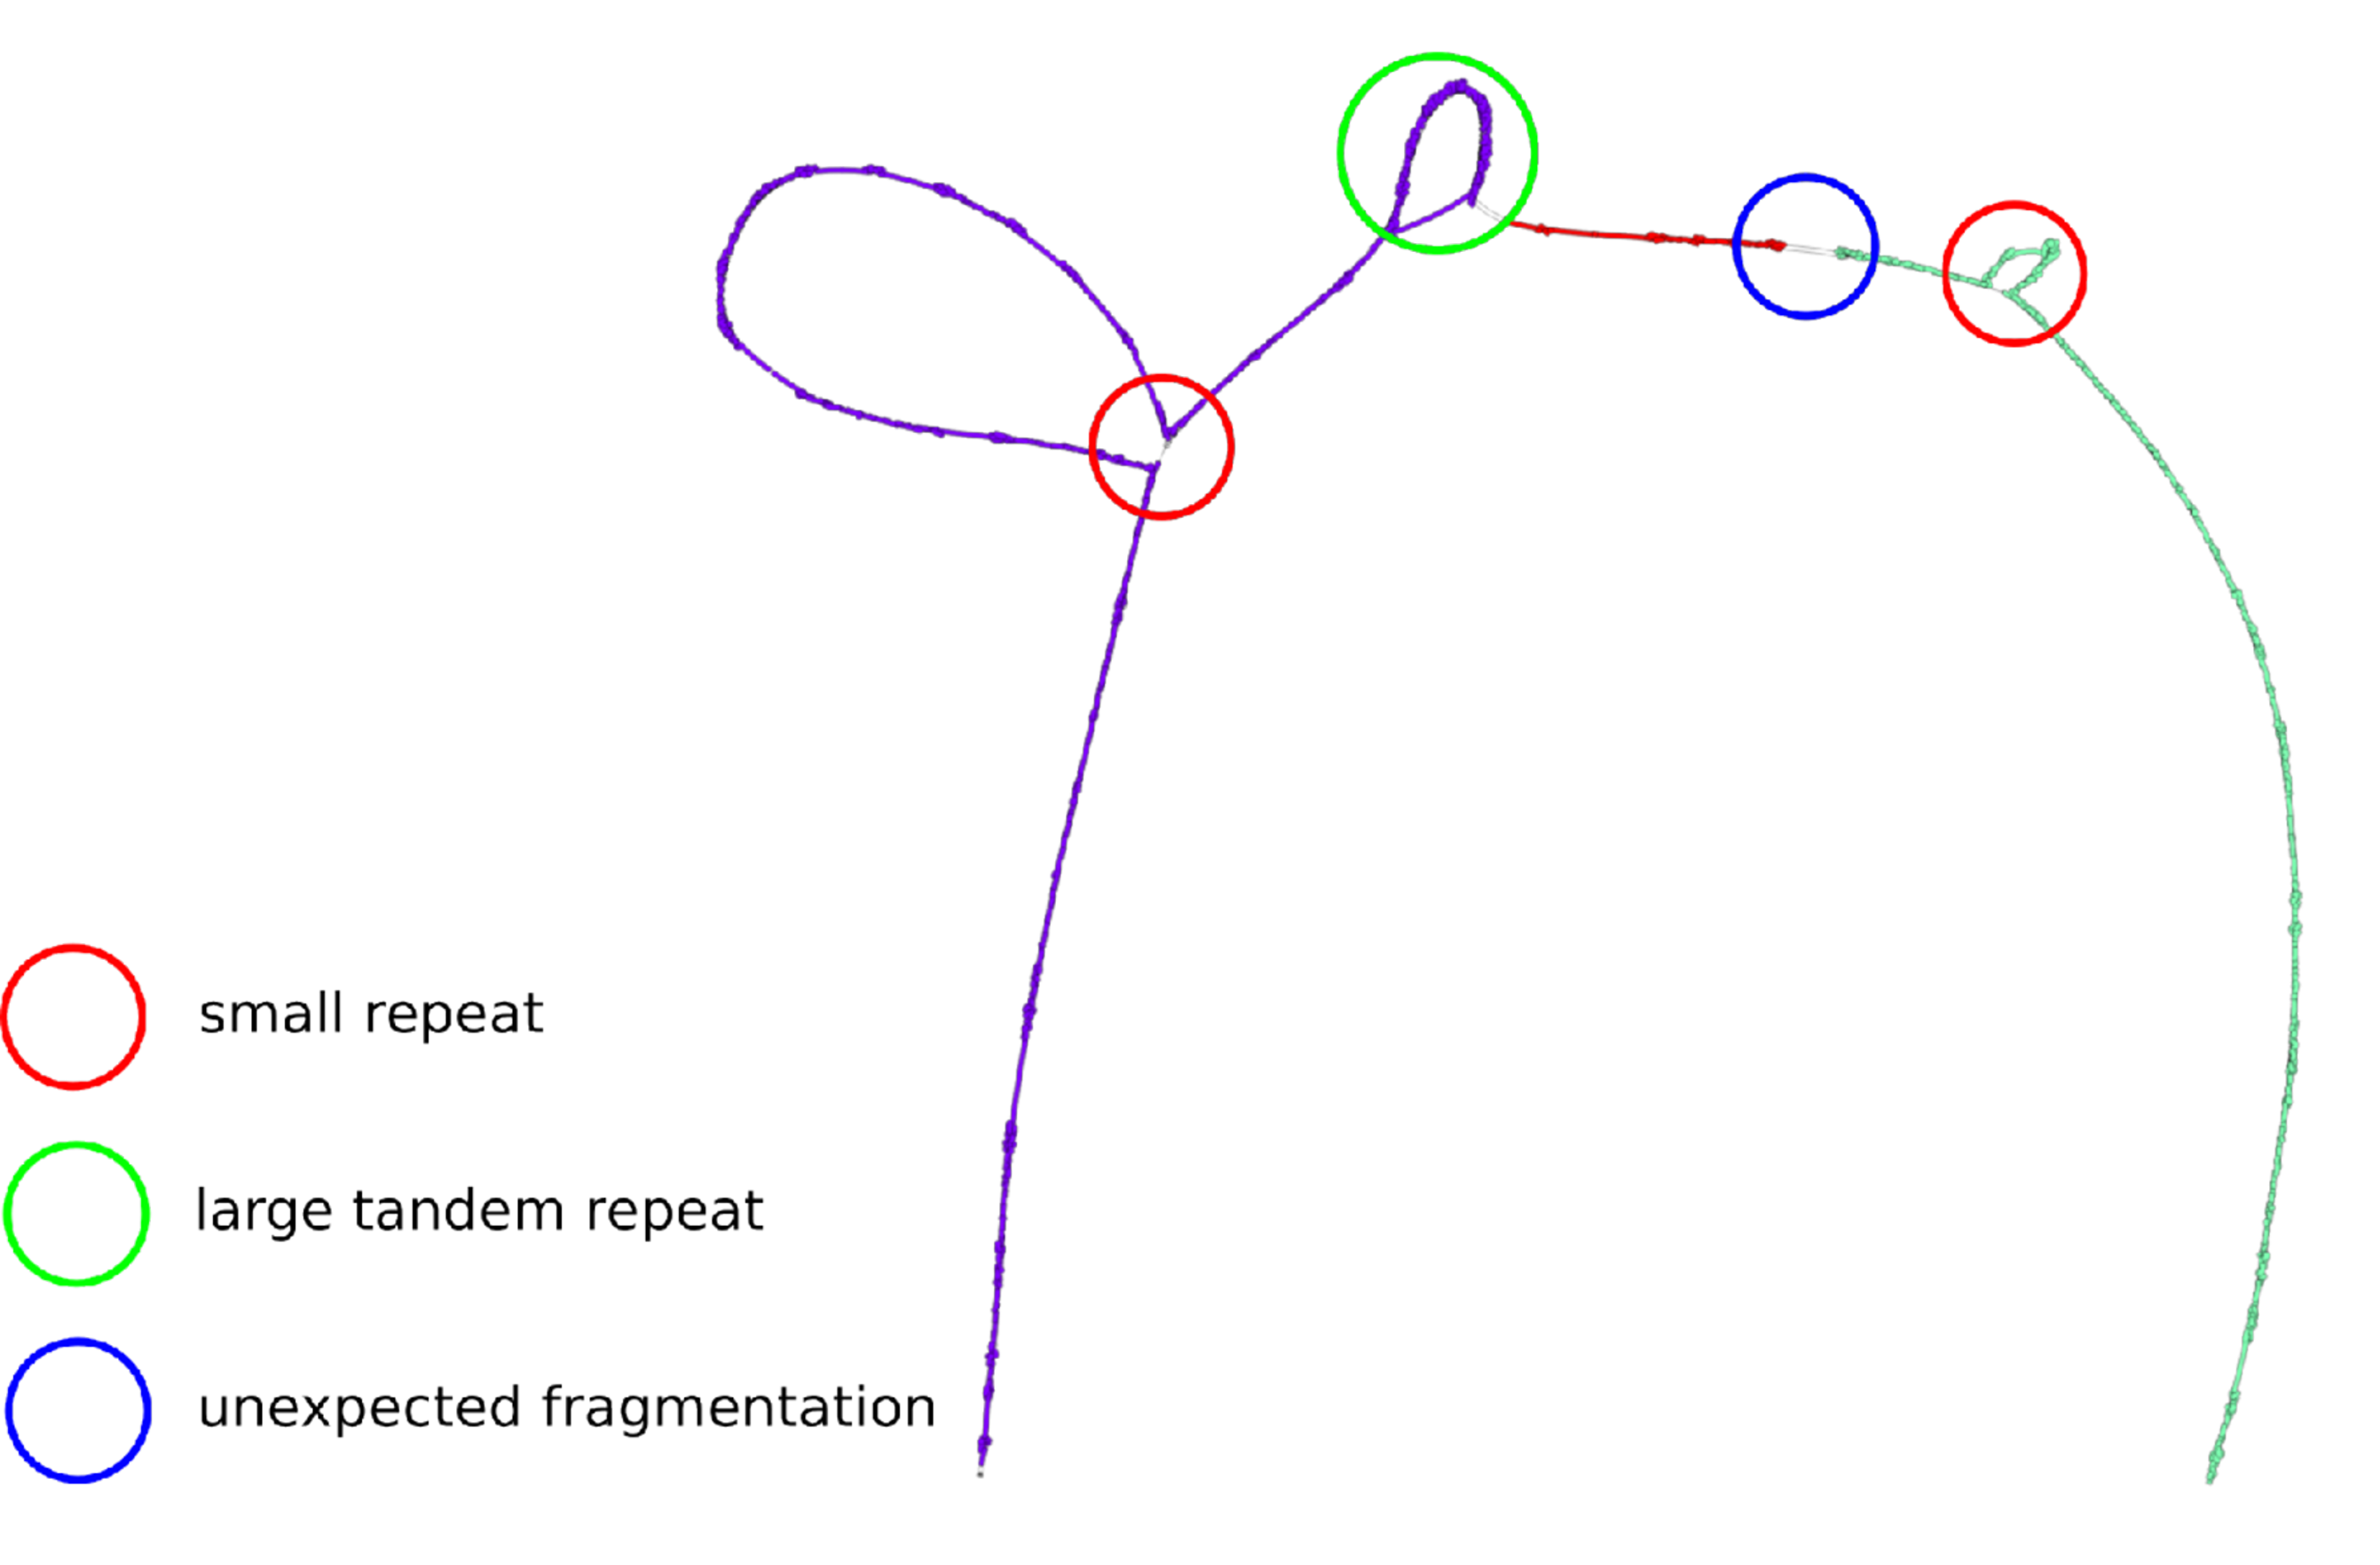
\includegraphics[width=\textwidth]{postassembly/images/t_roseus_projection_annoted.pdf}
    \caption{This graph was the overlap graph (found by \minimap), read used by \canu to build a contigs was are colored with same color. We can observe 2 fragmentation point, one can be explain by a repetition, green circle, we can observe repetition solved by \canu, but the fragmentation between green and red can't be explain by a repetition.}
    \label{postassembly:fig:t_roseus_example}
\end{figure}

In Figure \ref{postassembly:fig:t_roseus_example} in fact we present the main idea of \knot combine information of assembly (the read coloration) with a maximum of information can be extract from reads (the \OLC graph build from \minimap). The information from contigs help us to ignore some already solve problem (red circle), unsolvable trouble (greed circle), to focus on strange situation (blue circle). Figure \ref{postassembly:fig:t_roseus_example} show a very simple example in real case the \OLC graph cann't be readable. For thes reason and to run analysis without an human eye we automatise the idea of \knot in a simple tools.

The paper was publish originally publish in Bioinformatics (\url{https://doi.org/10.1093/bioinformatics/btz219}), we reformat the paper in the style of this current document for reasons of readability.

\subfile{paper/knot.tex}

\subfile{paper/misassemblies-in-noisy-assemblies.tex}

\section{Conclusion}

In this paper we show the idea to go back to raw read information, could be very help full for bacterial assembly. To use \knot on more complex dataset we need improve some part of \knot, especially the construction of the graph, its representation in memory and the search of paths between contigs extremity. This improvement required some code writing, but the original idea of comme back to raw read information can be used for more genome assembly improvement. I present this idea, in my conclusion.


\onlyinsubfile{
\bibliographystyle{plainnat}
\bibliography{main}
\addcontentsline{toc}{chapter}{Bibliography}
}

\end{document}